\begin{frame}
  \begin{center}
    \large{1. Support Vector Machines}
  \end{center}
\end{frame}

% \subsection{Support Vector Machines (SVM) and kernel methods}
% \begin{frame}[plain,c]
% \begin{center}
% \Huge Support Vector Machines
% \end{center}
% \end{frame}

\begin{frame}{1.1 SVM: le principe}
  \begin{figure}[htb]
    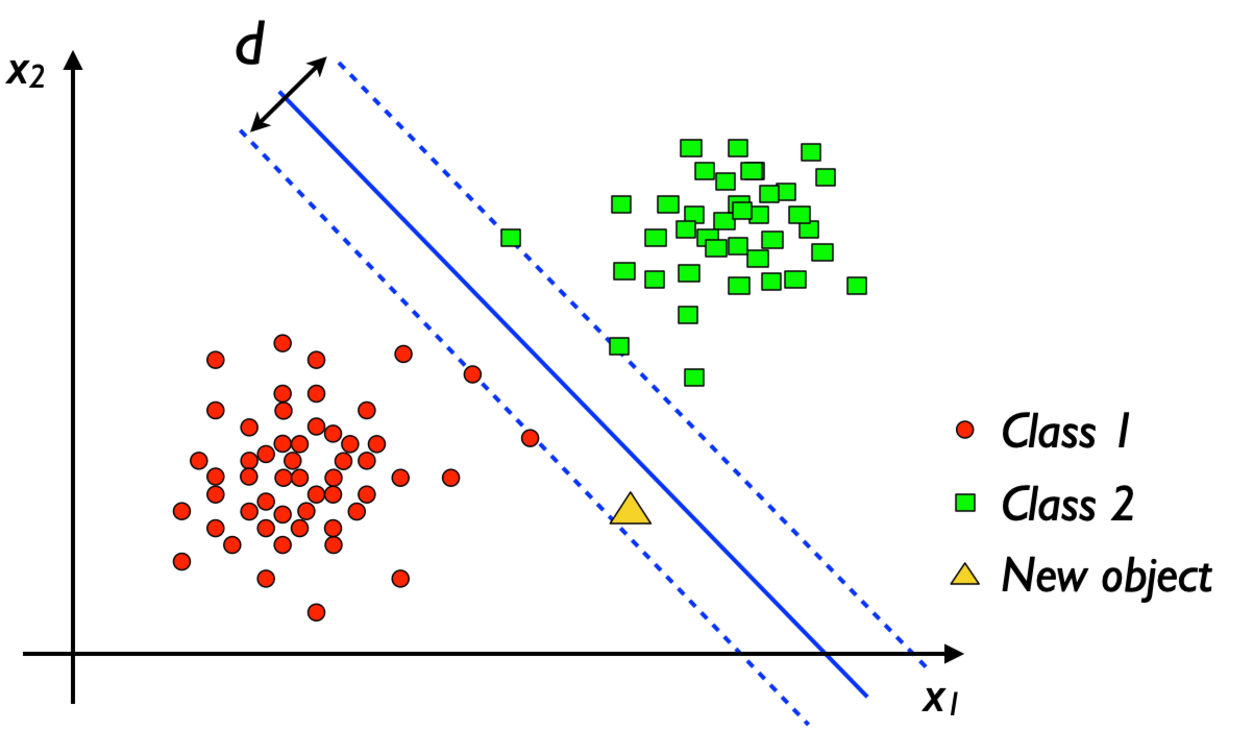
\includegraphics[width=0.5\textwidth]{figures/SVM_general.pdf}
  \end{figure}
  \begin{itemize}
    \item Pour des données linéairement séparables, on place un ruban entre les données. 
    \item L'épaisseur $d$ de ce ruban est à maximisier. 
  \end{itemize}
\end{frame}

\begin{frame}{1.2 SVM: le cas séparable}
  \begin{figure}[htb]
    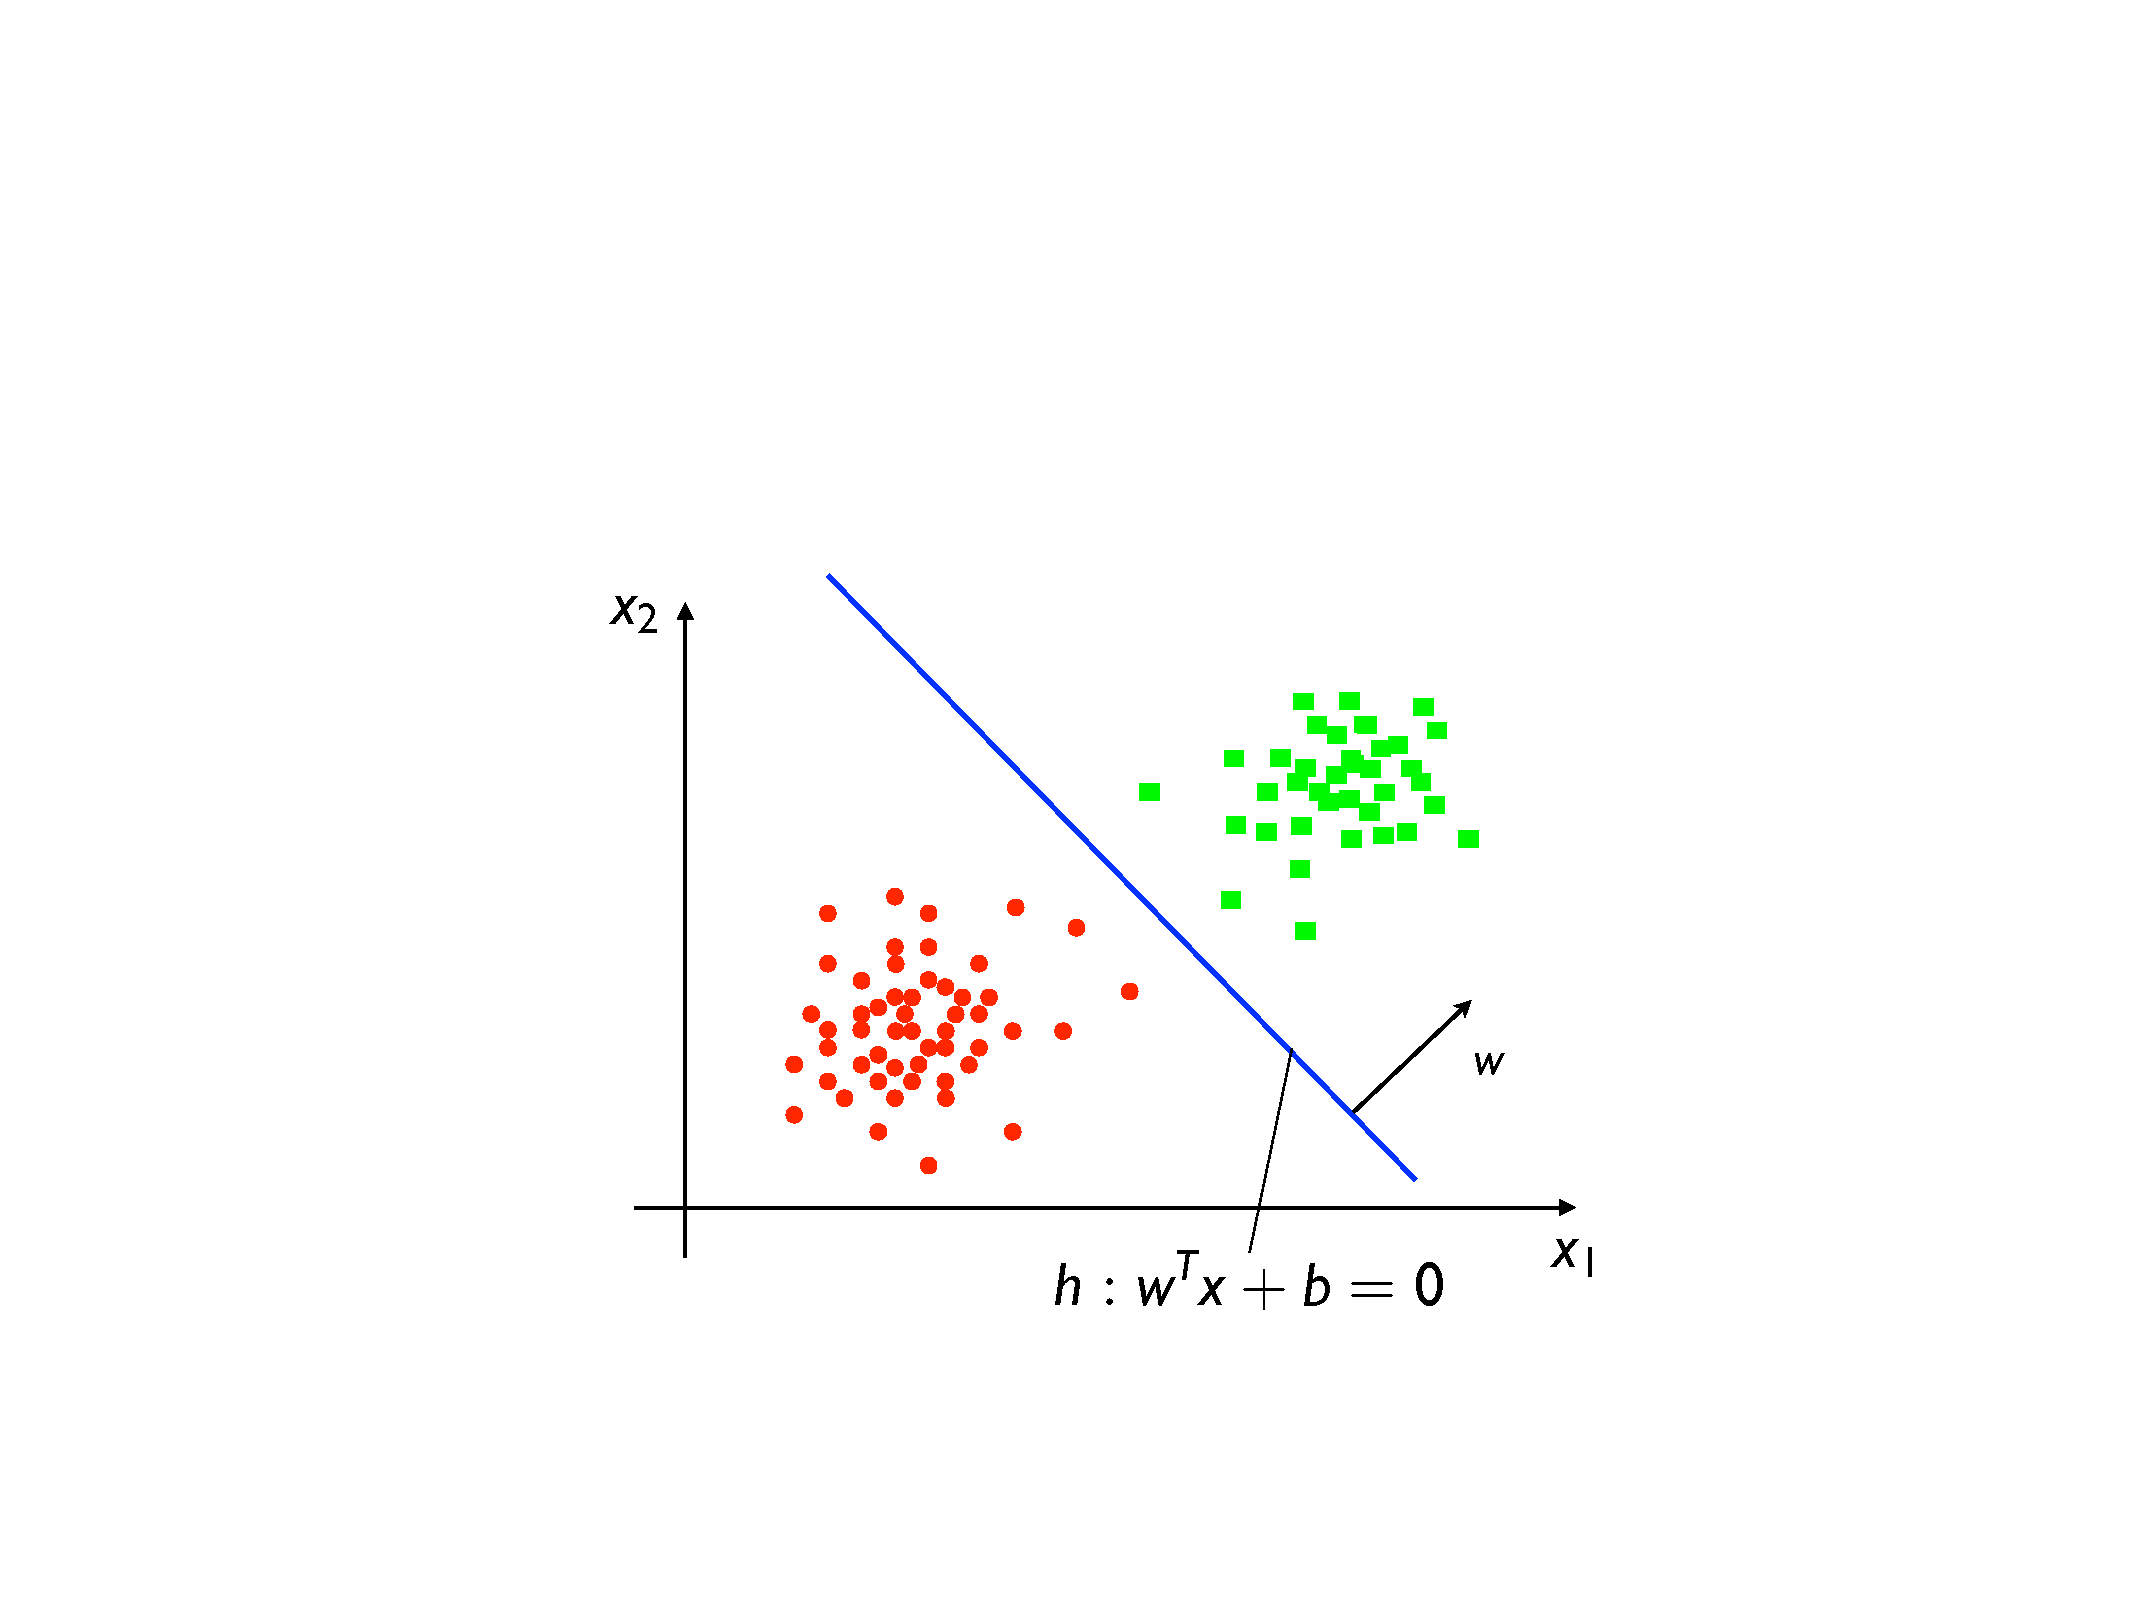
\includegraphics[width=0.6\textwidth]{figures/SVM_1a.pdf}
  \end{figure}
  \begin{itemize}
    \item Hyperplan séparateur $h: \langle \overrightarrow{w};\overrightarrow{x} \rangle + b = 0$.
    \item $\overrightarrow{w}$: vecteur normal de l'hyperplan séparateur. $b$ est le biais (intercept). 
    \item $\langle\overrightarrow{w};\overrightarrow{x} \rangle$ est le produit scalaire du vecteur normal (vecteur des poids) avec le vecteur des descripteurs. 
    \item Pour des descripteurs centrés réduits, $\overrightarrow{w}$ reflète l'importance des descripteurs.
  \end{itemize}
\end{frame}

\begin{frame}{1.2 SVM: le cas séparable}
  \begin{figure}[htb]
    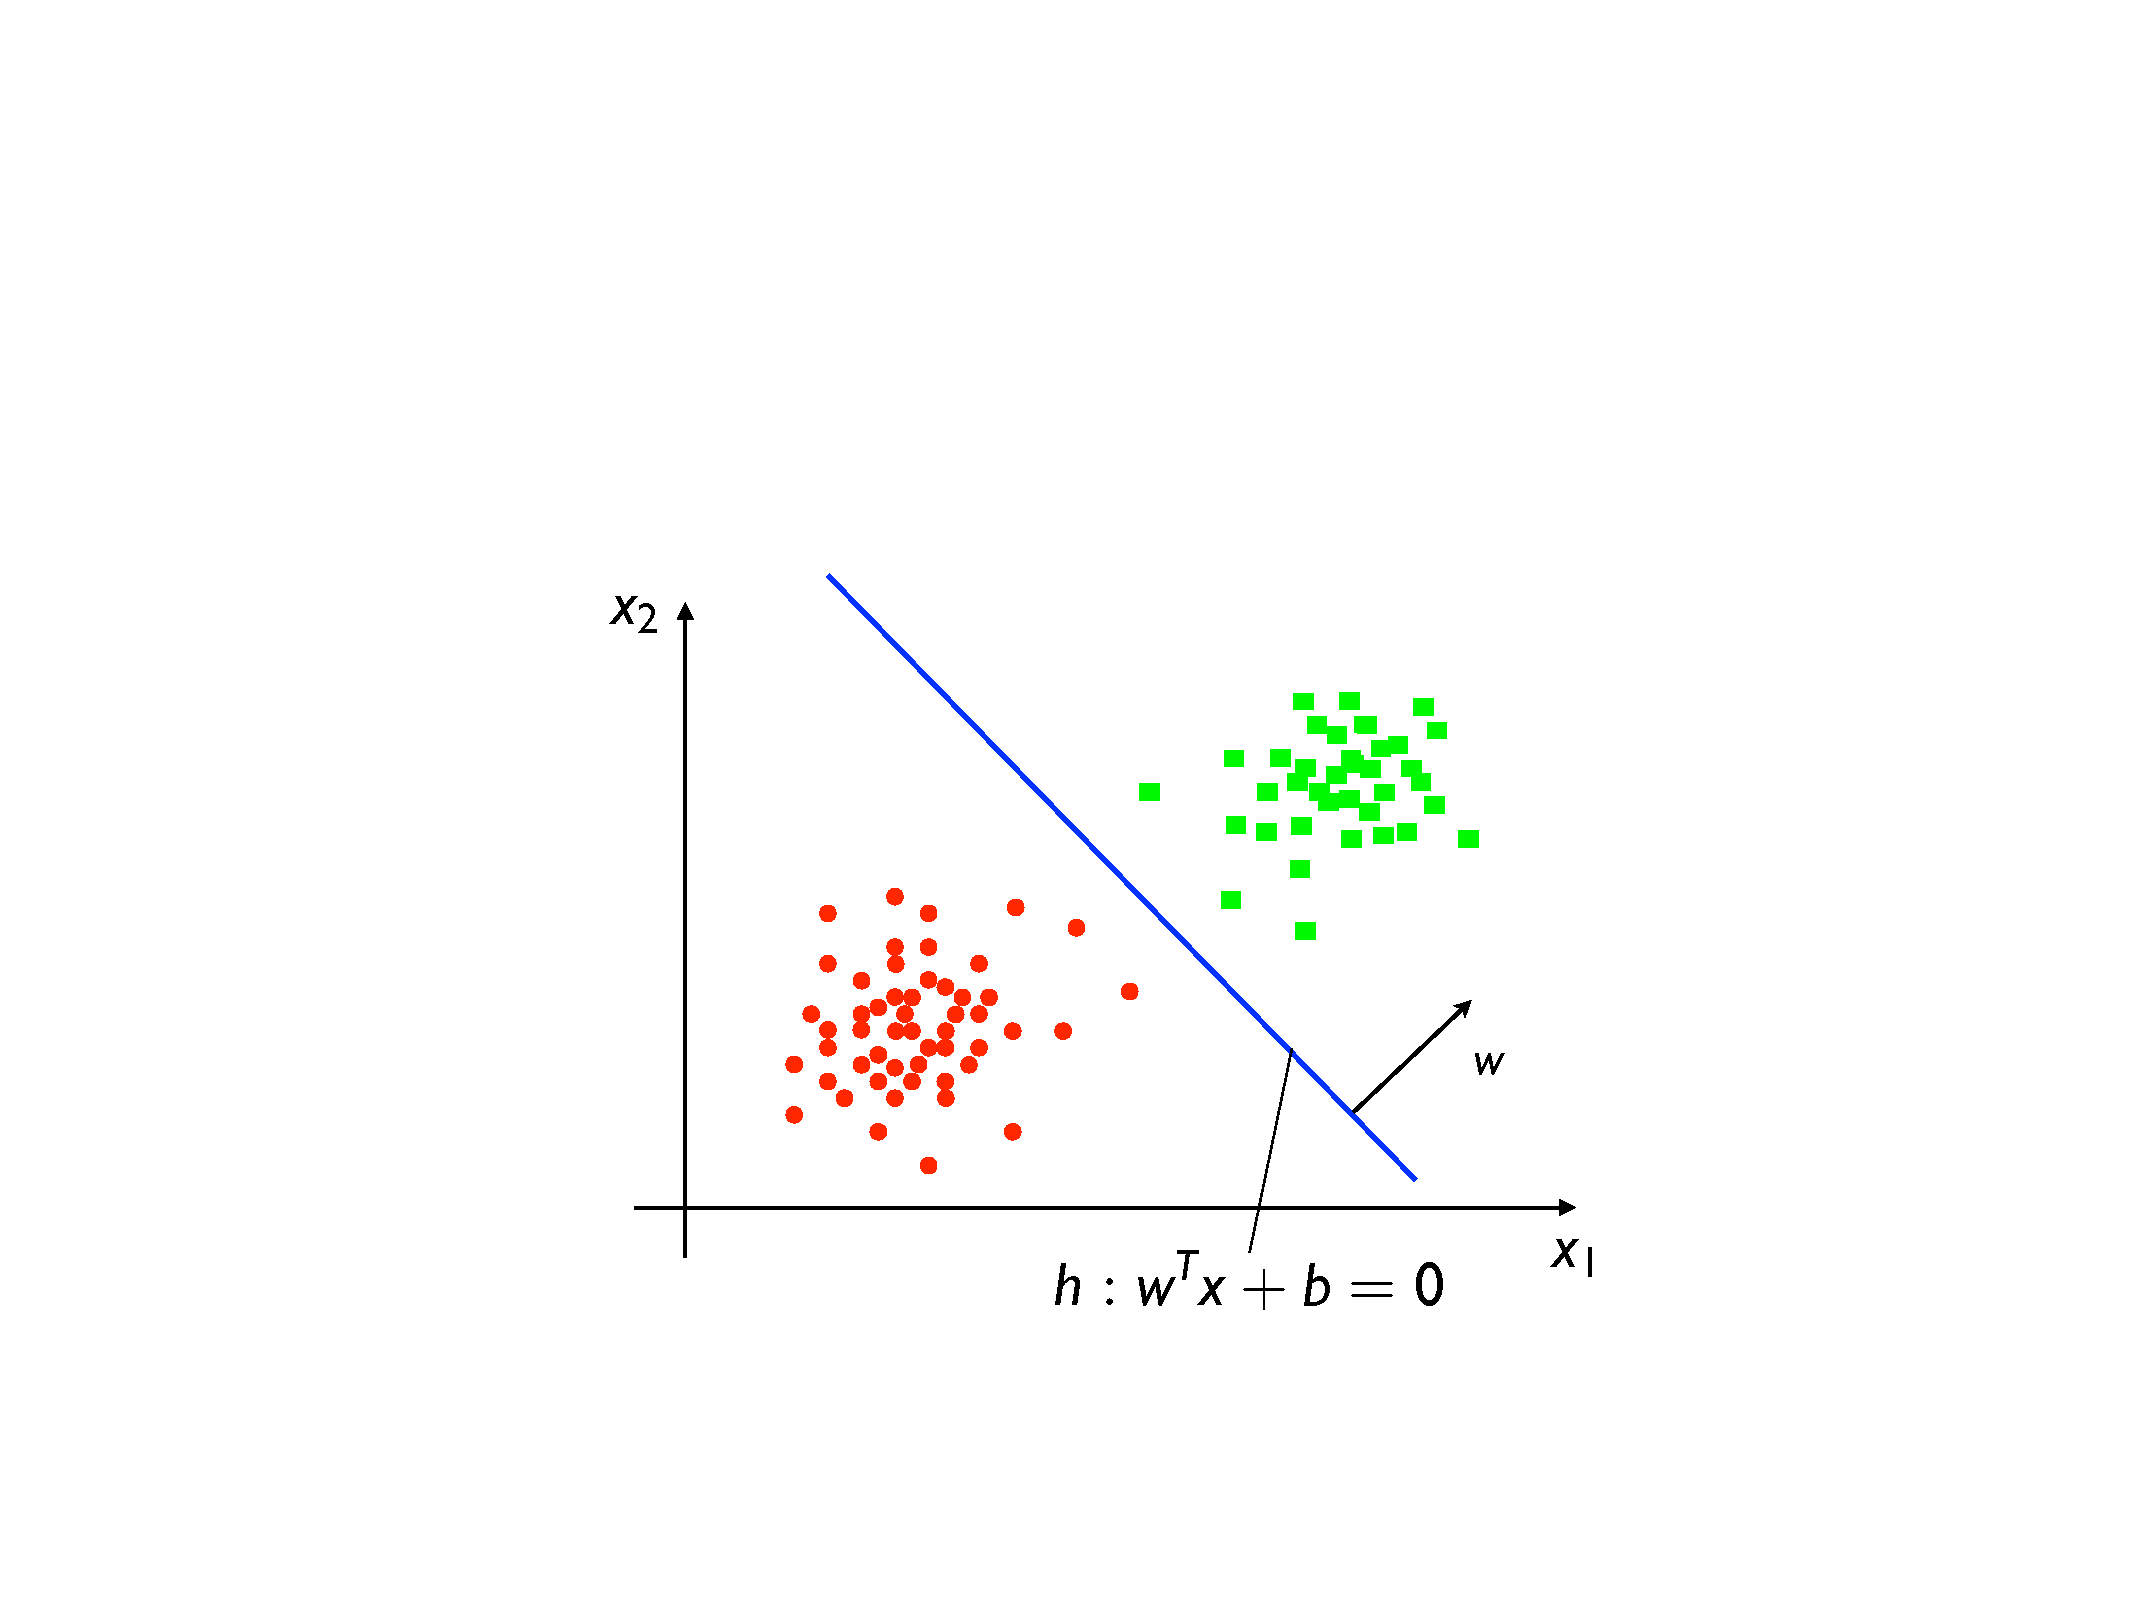
\includegraphics[width=0.6\textwidth]{figures/SVM_1a.pdf}
  \end{figure}
  \begin{itemize}
    \item $\langle\overrightarrow{w},\overrightarrow{x} \rangle + b  > 0$: $\overrightarrow{x}$ se trouve du côté vers lequel $\overrightarrow{w}$ pointe. 
    \item $\langle \overrightarrow{w}, \overrightarrow{x} \rangle + b  < 0$: $\overrightarrow{x}$ se trouve du côté opposé. 
    \item Avec l'encodage $y\in\{-1,+1\}$, un échantillon $\overrightarrow{x_i}$ est correctement classifié si $y_i(\langle \overrightarrow{w};\overrightarrow{x_i} \rangle + b) > 0$.
  \end{itemize}
\end{frame}

\begin{frame}{1.2 SVM: le cas séparable}
  \begin{figure}[htb]
    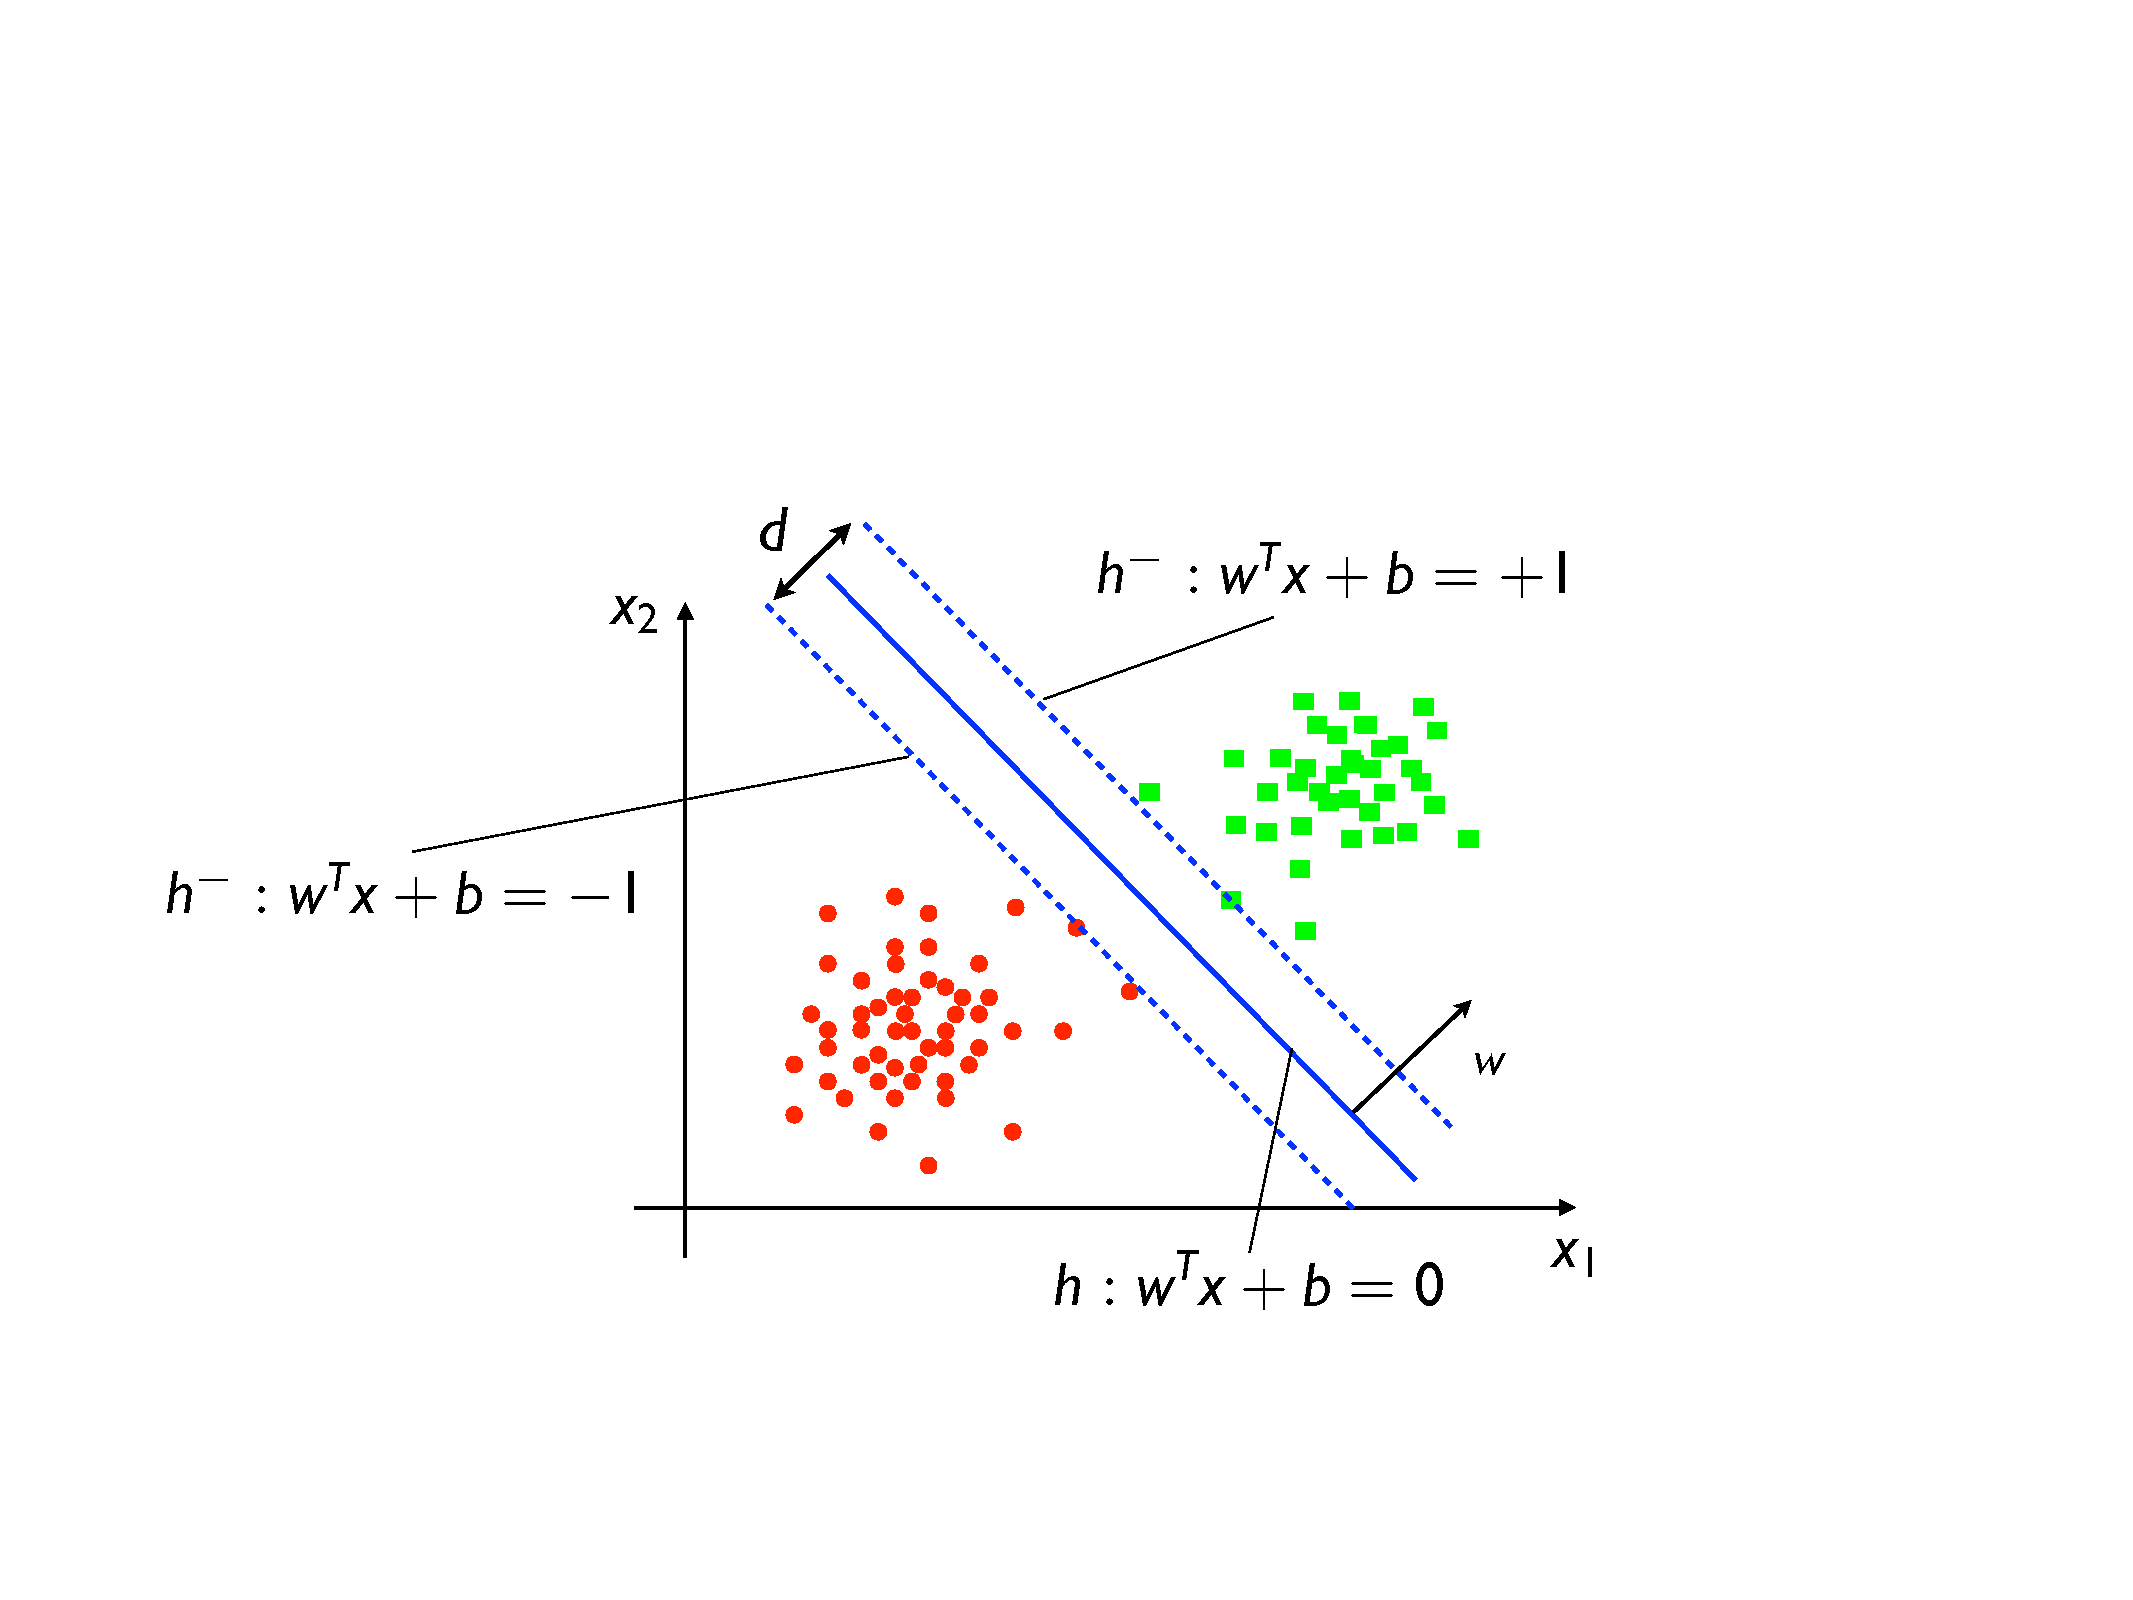
\includegraphics[width=0.6\textwidth]{figures/SVM2.pdf}
  \end{figure}
  \begin{itemize}
    \item Le ruban est défini par deux hyperplans parallèles, pour lesquels $\langle \overrightarrow{w};\overrightarrow{x} \rangle + b = \pm 1$ 
    \item La distance entre ces deux hyperplans $\langle \overrightarrow{w};\overrightarrow{x} \rangle + b = \pm 1$ est : 
    \begin{equation}
      d = \frac{2}{\|\overrightarrow{w}\|}
    \end{equation}
    \item Maximiser $d$ est équivalent à minimiser $\|\overrightarrow{w}\|^2$.
  \end{itemize}
\end{frame}


\begin{frame}{1.2 SVM: le cas séparable}
  \begin{figure}[htb]
    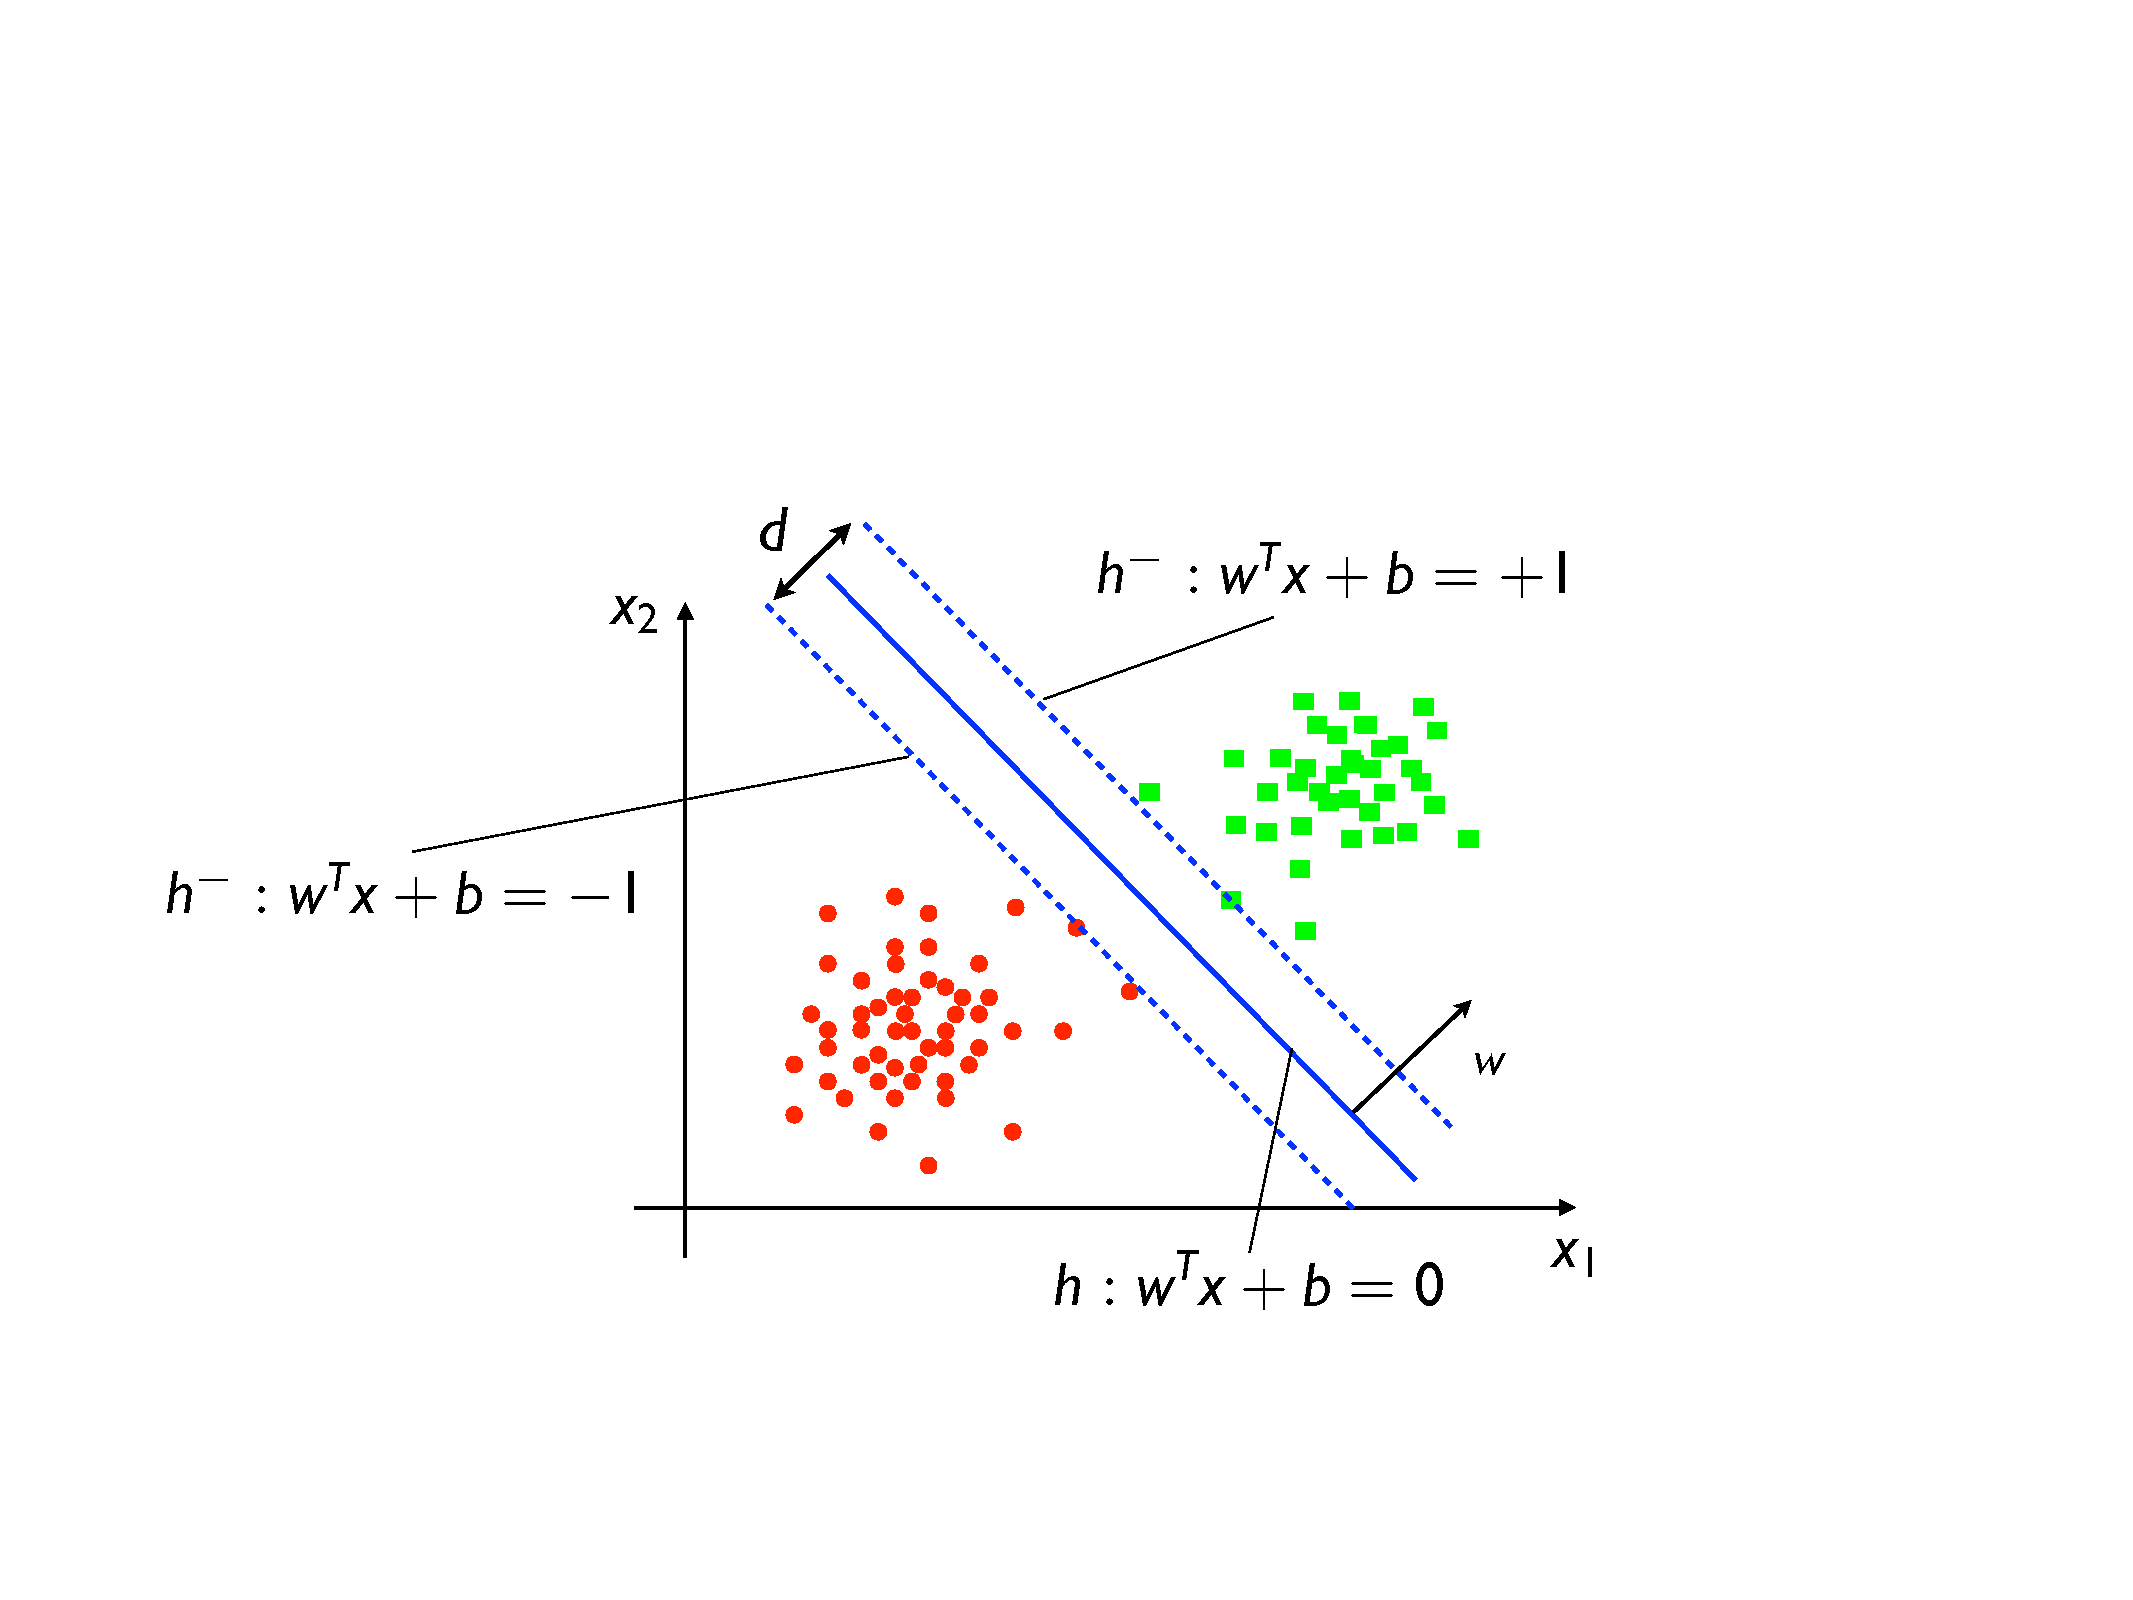
\includegraphics[width=0.6\textwidth]{figures/SVM2.pdf}
  \end{figure}
  \begin{itemize}
    \item Cela mène à un problème d'\textbf{optimisation convexe sous contraintes} : 
    \begin{eqnarray*}
      \mbox{minimize} & & \|\overrightarrow{w}\|^2 \\
      \mbox{subject to} & & y_i(\langle \overrightarrow{w};\overrightarrow{x_i} \rangle + b) \geq 1 \quad i = 1, \ldots, N
    \end{eqnarray*}
    \item La convexité implique qu'il n'y a pas de minimum local en dehors du minimum global. 
  \end{itemize}
\end{frame}


\begin{frame}{1.3 SVM pour le cas non-séparable}
  \begin{figure}[htb]
    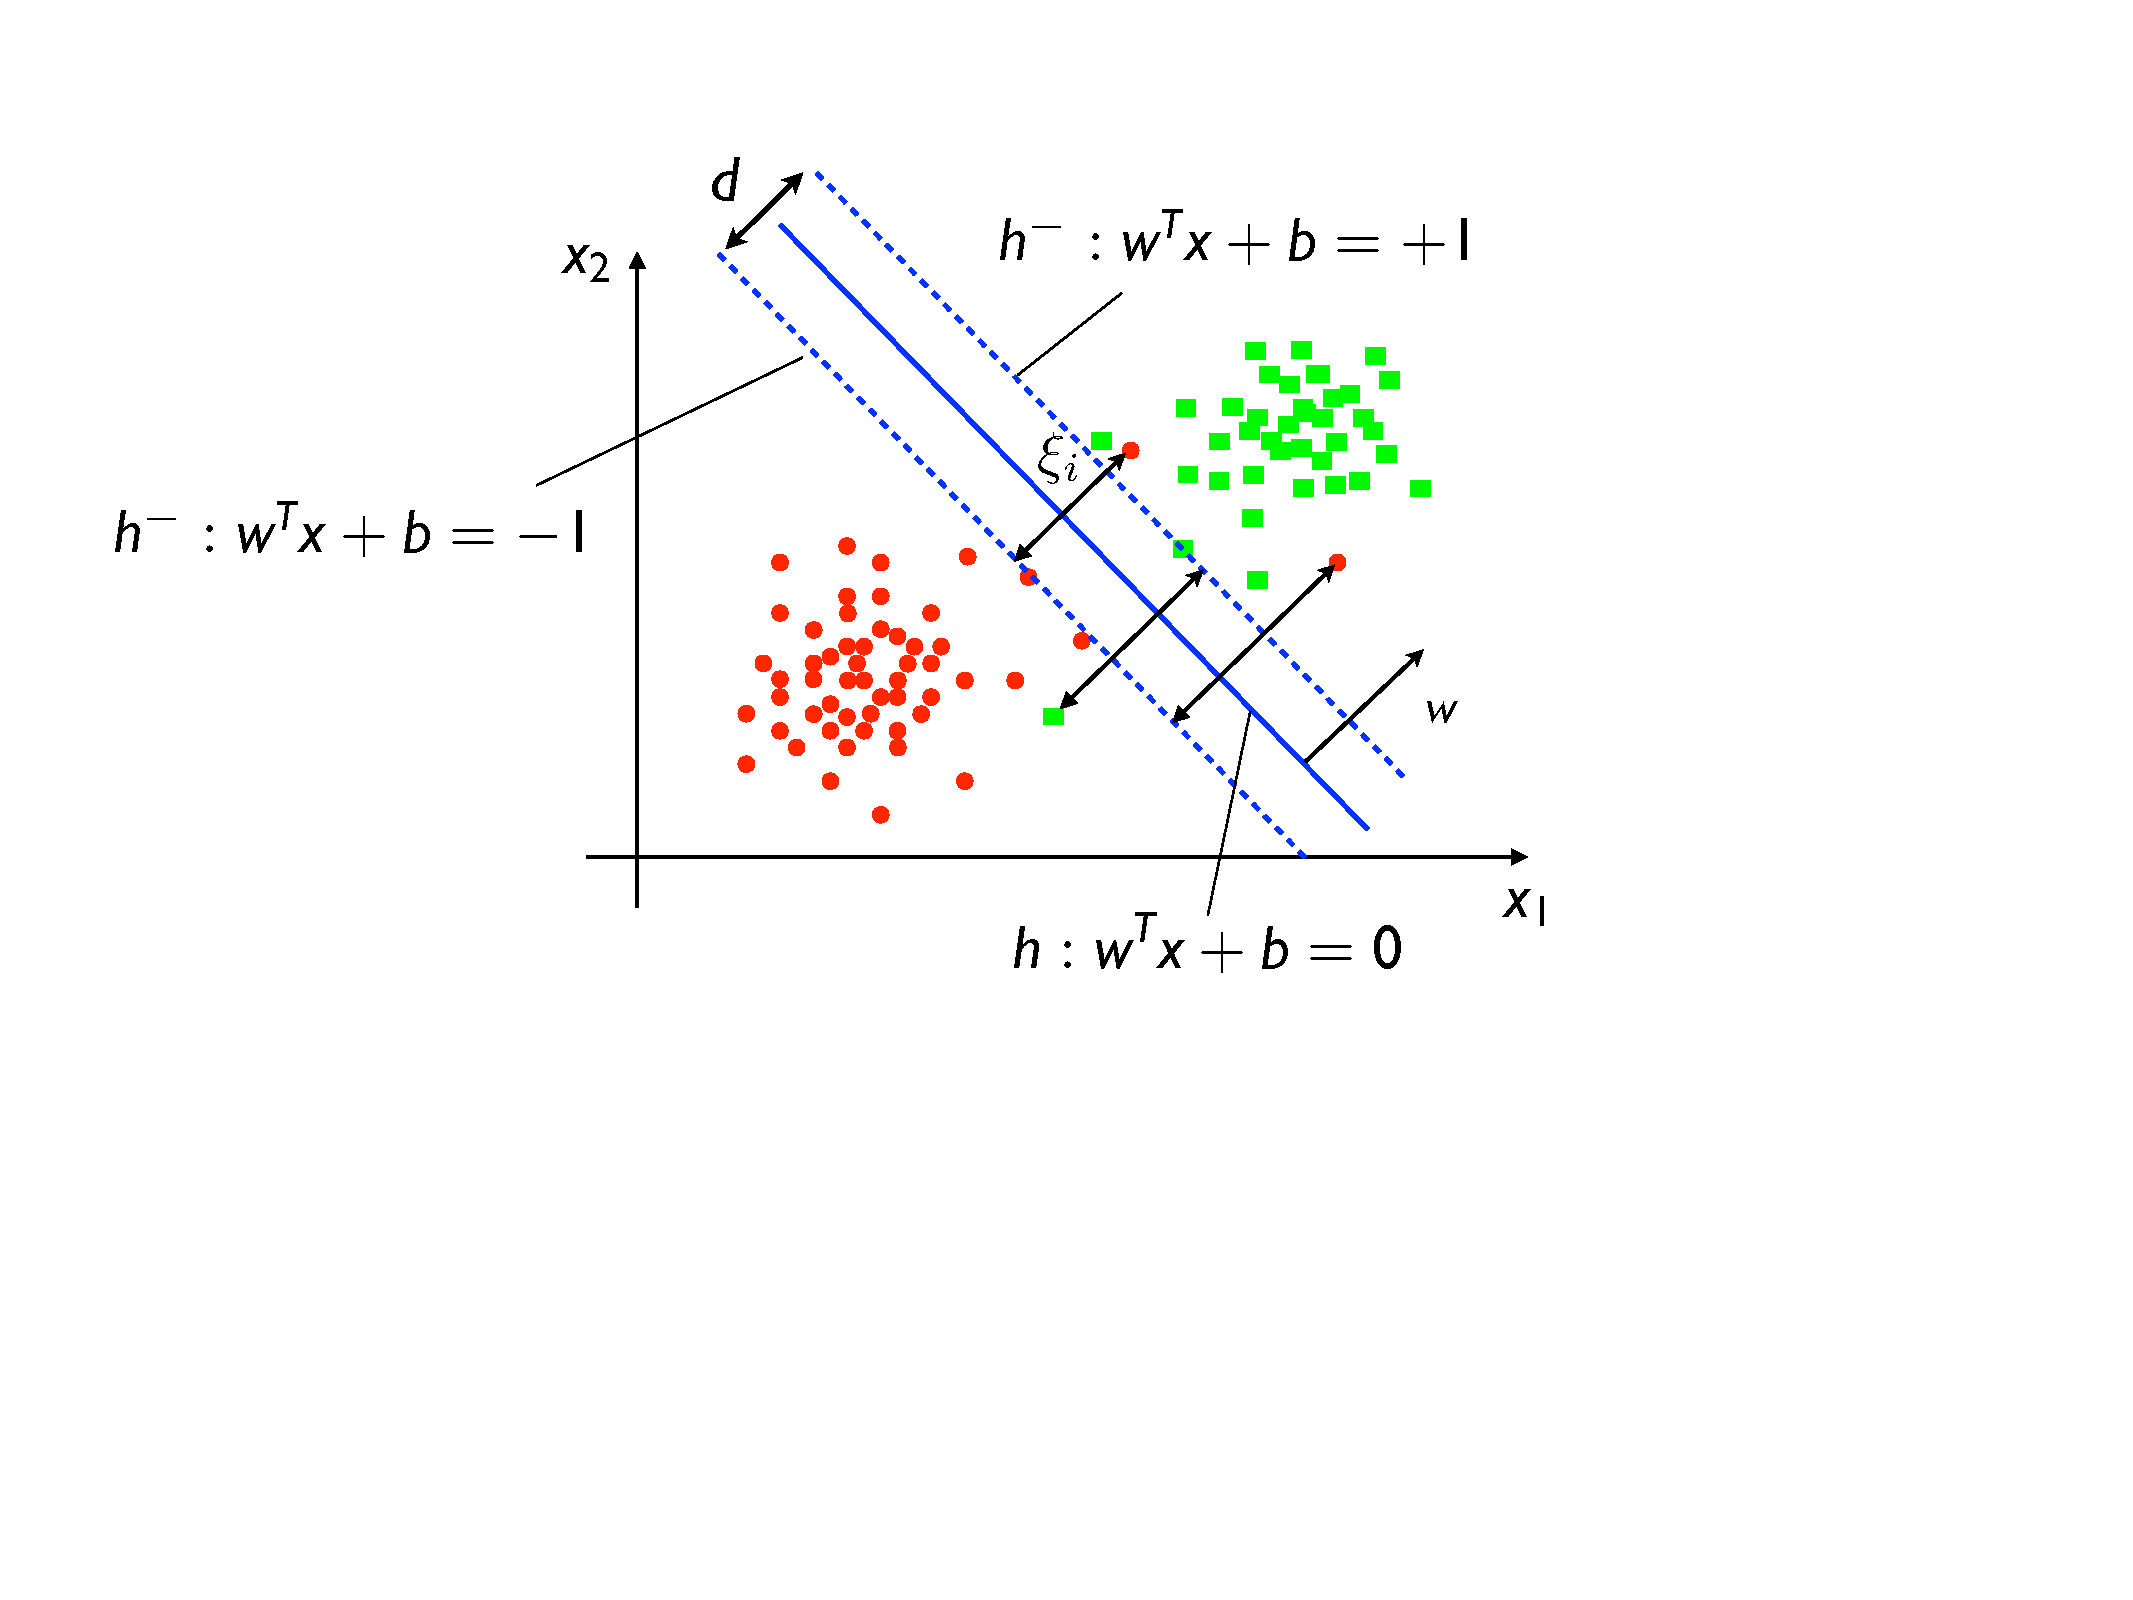
\includegraphics[width=0.6\textwidth]{figures/SVM3.pdf}
  \end{figure}
  \begin{itemize}
    \item Si les données ne sont pas séparables, il faut trouver un compromis entre l'erreur $\sum_{i=1}^{N}\xi_i$ et la régularisation $\|\overrightarrow{w}\|^2$:
    \begin{eqnarray*}
      \min_{\overrightarrow{w},\xi} & & \|\overrightarrow{w}\|^2 + C \sum_{i=1}^{N}\xi_i\\
      \mbox{subject to} & & y_i(\langle \overrightarrow{w};\overrightarrow{x_i} \rangle + b) \geq 1 - \xi_i \quad i = 1, \ldots, N \\
      & & \xi_i \geq 0 \quad i = 1, \ldots, N
    \end{eqnarray*}
    % \begin{equation*}
    %   \min_{w,\xi} \|w\|^2 + C \sum_{i=1}^{N}\xi_i
    % \end{equation*}
    %\item This corresponds to the general formulation we have seen before.
    % \begin{equation*}
    %   \param ^{\ast} = \argmin_{\param} \loss (\param) + \lambda \mathcal{R}(\param)
    % \end{equation*}
    %\item Normal vector $w$: vector of feature weights.
    %\begin{equation*}
    % f(x) = w^Tx + b = \sum_{k=1}^{P}w^{(k)}x^{(k)} + b
    %\end{equation*}
  \end{itemize}
\end{frame}

\begin{frame}{1.4 Solution}
  \begin{itemize}
    \item La solution du problème d'optimisation implique le formalisme Lagrangian. 
    \item On obtient une solution pour $\overrightarrow{w}$ : 
    \begin{equation*}
      \overrightarrow{w} = \sum_{i=1}^N\alpha_iy_i\overrightarrow{x_i}
    \end{equation*}
    ce qui donne l'équation de l'hyperplan : 
    \begin{eqnarray*}
      f(\overrightarrow{x}) &=& \sum_{i=1}^N\alpha_iy_i\langle \overrightarrow{x_i}, \overrightarrow{x} \rangle + b\\
      &=& \sum_{\overrightarrow{x_i} \in SV}\alpha_iy_i\langle \overrightarrow{x_i}, \overrightarrow{x} \rangle + b
    \end{eqnarray*}
    \item $SV$ est l'ensemble des vecteurs de support : des vecteurs qui sont situés sur le "ruban". 
  \end{itemize}
\end{frame}

\begin{frame}{1.4 Solution - Observations}
  \begin{equation*}
  f = \sum_{\overrightarrow{x_i} \in SV}\alpha_iy_i\langle \overrightarrow{x_i}, \overrightarrow{x} \rangle + b
  \end{equation*}
  \begin{enumerate}
    \item La décision ne dépend que d'un faible nombre d'observations.
    \item La décision ne dépend que de produits scalaires entre $\overrightarrow{x_i}$ et $\overrightarrow{x}$. 
  \end{enumerate}
\end{frame}



% \begin{frame}{SVM for not linearly separable data}
%   \begin{itemize}
%     \item SVM correspond to the following constrained optimization problem:
%     \begin{eqnarray*}
%       \min_{w,\xi} & & \|w\|^2 + C \sum_{i=1}^{N}\xi_i\\
%       \mbox{subject to} & & y_i(w^Tx_i + b) \geq 1 - \xi_i \quad i = 1, \ldots, N \\
%       & & \xi_i \geq 0 \quad i = 1, \ldots, N
%     \end{eqnarray*}
%     \item This problem can be efficiently solved with the Lagrange formalism (not shown).
%     \item We note that this corresponds to the formulation we have seen earlier:
%     \begin{equation*}
%       \param ^{\ast} = \argmin_{\param} \loss (\param) + \lambda \mathcal{R}(\param)
%     \end{equation*}
%   \end{itemize}
% \end{frame}

\begin{frame}{1.5 SVM: Au delà du linéaire}
  \begin{figure}[htb]
    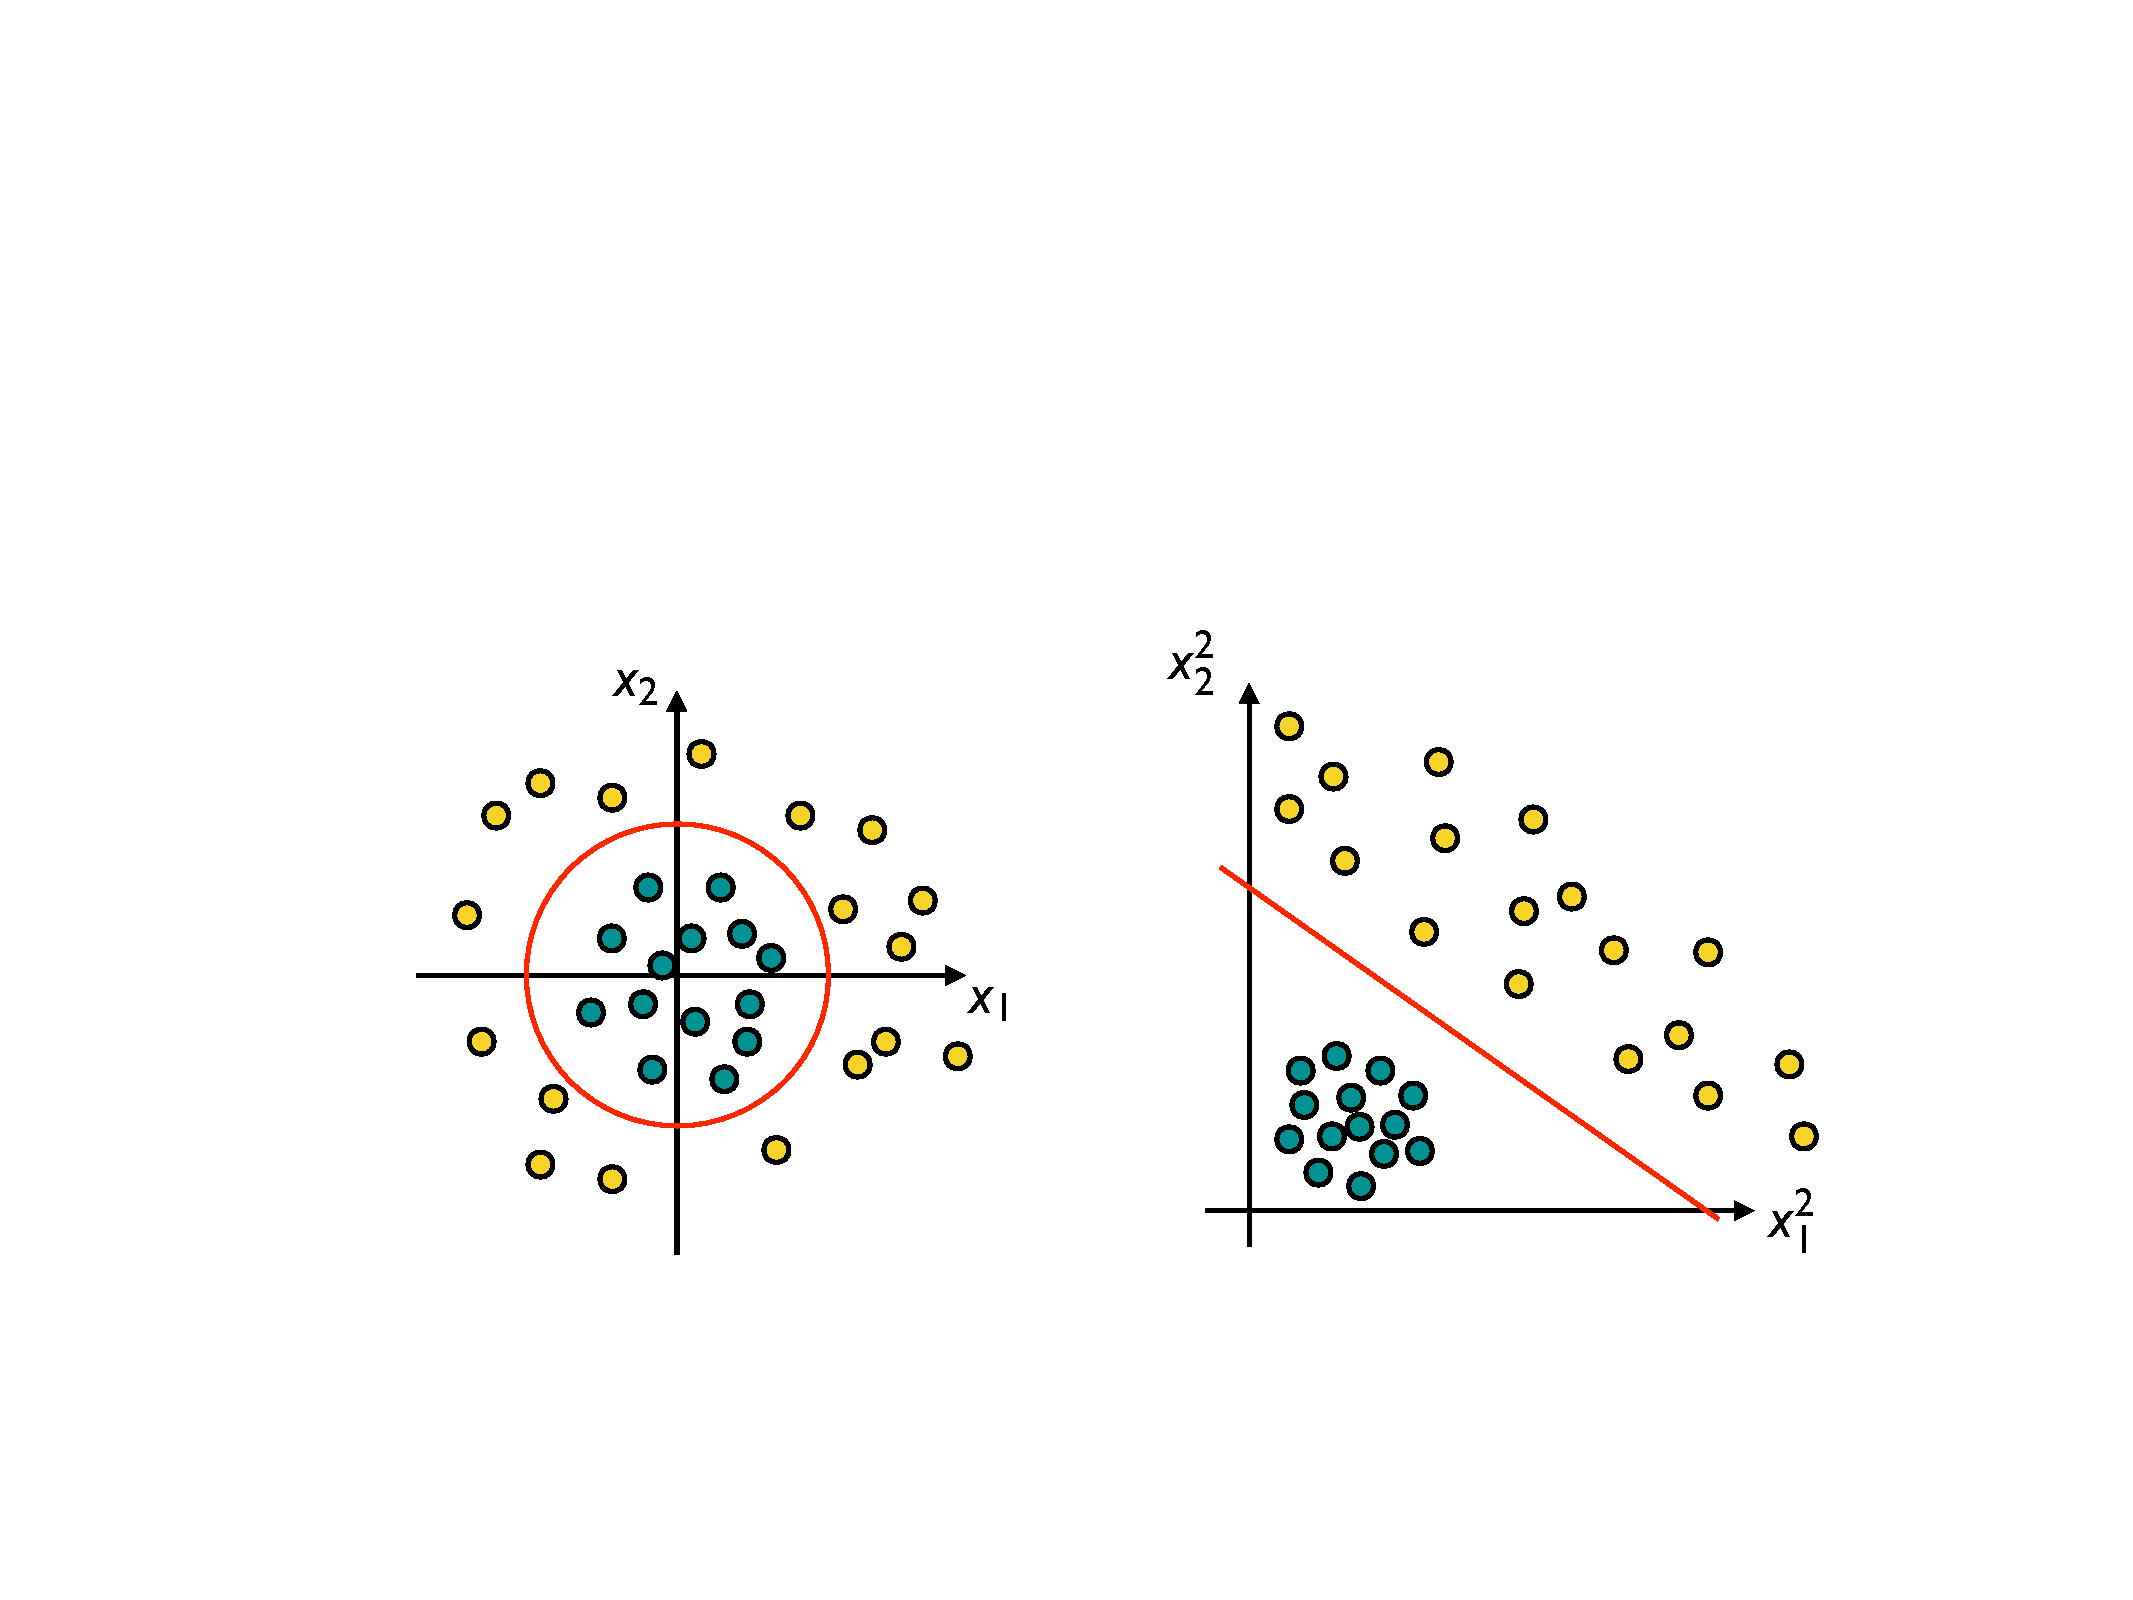
\includegraphics[width=0.6\textwidth]{figures/KernelTrick.pdf}
  \end{figure}
  \begin{itemize}
    \item Limitation: classifieur linéaire
    \item Solution: transformer $\overrightarrow{x}$ dans un espace à plus haute dimension.
    \item SVM: cette transformation peut être faite de manière implicite par la méthode de noyaux. 
  \end{itemize}
\end{frame}


\begin{frame}
  \begin{center}
    \large{2. Méthode de noyaux}
  \end{center}
\end{frame}


\begin{frame}
  \frametitle{Produit scalaire}
  \begin{itemize}
  \item $\langle \xvec, \xvec^\prime \rangle = \sum_{j=1}^p x_j x_j^\prime$
  \item $\langle \xvec, \xvec^\prime \rangle = \ltwonorm{\xvec} \ltwonorm{\xvec^\prime} \cos \theta$ \hspace{1em}
     $\ltwonorm{\xvec}^2 = \langle \xvec, \xvec \rangle$
  \item Interprétable comme \blue{mesure de similarité}
  \item \blue{Forme définie positive bilinéaire :}
    \begin{itemize}
    \item $\langle \xvec, \xvec^\prime \rangle = \langle \xvec^\prime, \xvec \rangle$
      pour tout $\xvec, \xvec^\prime \in \mathcal{X}$
    \item $\langle \xvec + \zvec, \xvec^\prime \rangle = \langle \xvec, \xvec^\prime \rangle +
      \langle \zvec, \xvec^\prime \rangle$       pour tout $\xvec, \xvec^\prime, \zvec \in \mathcal{X}$
    \item $\langle a \xvec, \xvec^\prime \rangle = a \langle \xvec, \xvec^\prime \rangle$ pour tout $a \in \RR$
    \item $\langle \xvec, \xvec \rangle \geq 0$ et $\langle \xvec, \xvec \rangle = 0 \text{ ssi } \xvec = 0$
    \end{itemize}
  \item Apparaît dans de nombreux algorithmes d'apprentissage.
  \end{itemize}
\end{frame}

\begin{frame}
  \frametitle{Noyau}
  \begin{itemize}
  \item \blue{Généralisation} du produit scalaire : $k: \xcal \times \xcal \rightarrow \RR$
    \begin{itemize}
    \item \blue{sémantiquement} une similarité
    \item \blue{mathématiquement} une forme définie positive 
    \end{itemize}
  \item Aronszajn: Si $k$ est semi-définie positive\footnote{Pour tout
      $m \in \NN^*$, pour tout
      $\{\xvec_1, \xvec_2, \dots, \xvec_m\} \in \xcal,$ la matrice
      $K \in \RR^{m \times m}$ telle que $K_{il} = k(\xvec_i, \xvec_l)$ est
      semi-définie positive}, il existe un espace de Hilbert $\hcal$ et une application
    $\varphi: \xcal \rightarrow \hcal$ telle que
    $\textcolor{MyOrange}{k(\xvec, \xvec^\prime) = \langle \varphi(\xvec), \varphi(\xvec^\prime)\rangle_{\hcal}}$
    pour tout $\xvec, \xvec^\prime, \zvec \in \mathcal{X}$
  \end{itemize}
\end{frame}

\begin{frame}
  \frametitle{Astuce du noyau}
  \begin{itemize}
    \item[]    $\textcolor{MyOrange}{k(\xvec, \xvec^\prime) = \langle \varphi(\xvec), \varphi(\xvec^\prime)\rangle_{\hcal}}$
    \item Si un algorithme ne fait intervenir les éléments de $\xcal$ que dans
      des produits scalaires, \blue{remplacer ces produits scalaires} par $k$ est
      équivalent à appliquer l'algorithme dans $\hcal$ après avoir appliqué
      $\varphi$
    \item Utile \blue{si $k$ est plus simple à calculer que $\varphi$}
      \pause
    \item Exemple : \blue{noyau quadratique}
      $k: (\xvec, \xvec^\prime) \mapsto (1 + \langle \xvec, \xvec^\prime \rangle)^2$
    \item[] Équivaut à $\varphi : (x_1, x_2, \dots, x_p) \mapsto (1, x_1, \dots, x_p,
      x_1^2, x_2^2, \dots, x_p^2, \sqrt{2} x_1 x_2, \dots, \sqrt{2}x_{p-1}x_p).$
  \end{itemize}
\end{frame}

\begin{frame}
  \frametitle{Régression ridge à noyau}
  \begin{itemize}
  \item \blue{Régression ridge :}
    {\footnotesize $\argmin_{\betavec \in \RR^{p+1}} \frac1n \left(\yvec - X \betavec \right)^\top
      \left(\yvec - X \betavec \right) + \lambda \ltwonorm{\betavec} $}      
    \begin{itemize}
    \item Solution : $\betavec^* = \left(X^\top X + \lambda I_p \right)^{-1} X^\top \yvec$
    \item Modèle : $f: \xvec \mapsto \langle \betavec^*, \xvec \rangle$
    \end{itemize}
  \item Reformulation :
    $f: \xvec \mapsto \textcolor{Aubergine}{\xvec X^\top} \left( \lambda I_n +
      \textcolor{MyPink}{XX^\top} \right)^{-1} \yvec $
    \pause
    \begin{itemize}
    \item $\textcolor{Aubergine}{\xvec X^\top} \in \RR^n$ a pour $i$-ème entrée :
      $\textcolor{Aubergine}{\langle \xvec, \xvec_i \rangle}$    
    \item $\textcolor{MyPink}{X X^\top} \in \RR^{n \times n}$ a pour entrée $(i,l)$ :
      $\textcolor{MyPink}{\langle \xvec_i, \xvec_l \rangle}$
    \end{itemize}
    \pause
  \item \blue{Kernelization :} remplacer $\textcolor{Aubergine}{\xvec X^\top}$ par
    $\textcolor{Aubergine}{\kappa} \in \RR^n$ tel que
    $\textcolor{Aubergine}{\kappa_i = k(\xvec, \xvec_i)}$ et $\textcolor{MyPink}{XX^\top}$ par
    $\textcolor{MyPink}{K} \in \RR^{n \times n}$ telle que $\textcolor{MyPink}{K_{il} = k(\xvec_i, \xvec_l)}$
  \item[] équivaut à transformer les données par $\varphi$ puis apprendre une régression ridge, \blue{pour environ le même coût algorithmique}
  \end{itemize}
\end{frame}

\begin{frame}
  \frametitle{Exemples de noyaux}
  \begin{itemize}
  \item \blue{Noyau quadratique} $k: (\xvec, \xvec^\prime) \mapsto (1 + \langle \xvec, \xvec^\prime \rangle)^2$
  \item[] $\varphi$ calcule tous les monômes de degré au plus 2 de $x_1, x_2, \dots, x_p$ 
    \pause
  \item \blue{Noyau polynomial} $k: (\xvec, \xvec^\prime) \mapsto (1 + \langle \xvec, \xvec^\prime \rangle)^d$
  \item[] $\varphi$ calcule tous les monômes de degré au plus $d$ de $x_1, x_2, \dots, x_p$ 
    \pause 
  \item \blue{Noyau RBF gaussien} $k: (\xvec, \xvec^\prime) \mapsto
    \exp\left( - \frac{\ltwonorm{\xvec - \xvec^\prime}^2}{\sigma^2} \right)$
  \item[] $\varphi$ calcule tous les monômes de $x_1, x_2, \dots, x_p$ 
  et $\hcal$ est de dimension infinie. 
  \end{itemize}
\end{frame}

% \begin{frame}
%   \frametitle{1.5 Exemples de noyaux}
%   \begin{itemize}
%   \item \blue{Noyau pour chaîne de caractères} $k: (\xvec, \xvec^\prime) \mapsto
%     \sum_{u \in \aset^m} \psi_u(\xvec) \psi_u(\xvec^\prime)$
%     \begin{itemize}
%     \item $\aset^m$ = l'ensemble des chaînes de $m$ caractères sur l'alphabet $\aset$
%     \item $\psi_u(\xvec) = 1$ si $u$ est une sous-chaîne de $\xvec$ et $0$ sinon.
%     \end{itemize}
%   \pause
%   \item $k(\xvec, \xvec^\prime)$ est le nombre de chaînes de $m$ caractères
%     communes à $\xvec$ et $\xvec^\prime$ et peut être calculé en
%     $\mathcal{O}(|\xvec|)$ au lieu de $\mathcal{O}(|\aset|^m)$.
%     \pause
%   \item Si $m=8$, $|\aset|=20$ et en moyenne $|\xvec| = 485,$ on compare 25,6 milliards
%     d'opérations à moins de 500.
%   \end{itemize}
% \end{frame}

% \begin{frame}
%   \begin{center}
%     \large{2. Machines à vecteurs de support}
%   \end{center}
% \end{frame}

% \begin{frame}[t]
%   \frametitle{2.1 Formulation primale}
%   \begin{itemize}
%   \item Classification binaire, $\ycal = \{-1, 1\}$ 
%   \[\argmin_{\betavec \in \RR^p, b \in \RR} \frac12 \ltwonorm{\betavec}^* + C \sum_{i=1}^n
%   \max\left( 0, 1 - y_i \left( \langle \betavec, \xvec_i \rangle + b \right)\right)\]
%   \end{itemize}
% \end{frame}

% \begin{frame}[t]
%   \frametitle{2.2 Formulation duale}
%     {\small \[\argmax_{\alphavec \in \RR^n} \sum_{i=1}^n \alpha_i - \frac12 \sum_{i=1}^n \sum_{l=1}^n
%       \alpha_i \alpha_l y_i y_l \langle \xvec_i, \xvec_l \rangle   \]}
%   \begin{itemize}
%   \item[] sous les contraintes $\sum_{i=1}^n \alpha_i y_i = 0$  et $0 \leq \alpha_i \leq C$ 
%   \item Modèle : $f: \xvec \mapsto \sum_{i=1}^n \alpha_i y_i \langle \xvec_i, \xvec \rangle$
%   \end{itemize}
% \end{frame}

% \begin{frame}[t]
%   \frametitle{2.3 SVR}
%   \begin{itemize}
%   \item Perte $\varepsilon$-insensible :
%     \[L(y, f(\xvec) = \max(0, |f(\xvec) - y| - \varepsilon)\]
%   \end{itemize}
% \end{frame}

%%% Local Variables:
%%% mode: latex
%%% TeX-master: "2022-01-azencott"
%%% End:
